\documentclass{article}
\usepackage{graphicx} % Required for inserting images
\usepackage{framed}
\usepackage{amsmath}
\usepackage{float}
\DeclareMathOperator\Arg{Arg}
\DeclareMathOperator{\arcsec}{arcsec}
\DeclareMathOperator{\arccot}{arccot}
\DeclareMathOperator{\arccsc}{arccsc}
\DeclareMathOperator{\trig}{trig}
\DeclareMathOperator{\arctrig}{arctrig}
\DeclareMathOperator{\Real}{Re}
\DeclareMathOperator{\Imag}{Im}
\usepackage{fancybox}
\usepackage{array}
\usepackage{amsmath}
\usepackage{amssymb}
\newcommand{\Mod}[1]{\ (\mathrm{mod}\ #1)}


\title{Satellite Problem}
\author{Aarush Chaubey}


\begin{document}

\maketitle

\doublebox{
    \parbox{\textwidth}{
    Problem Statement: 

    \vspace{2mm}
    A satellite is orbiting Earth in a circular path with variables as follows. Suppose the satellite was to be propelled to a location which would result in its total energy(potential and kinetic) being 0. Find the minimum amount of energy needed to achieve this. The energy is instantaneously applied, and the problem is considering the two-body system of the Earth and the satellite i.e. no Moon, Sun, etc...

    \vspace{2mm}
    
    m = Satellite mass\\
    M = Earth's mass\\
    R = initial radius above Earth\\
    G = gravitational constant\\
    E = Energy needed to propel the spaceship
    }
    }

\vspace{5mm}
To begin, we must first realize that the minimum energy required has to result from the satellite being ejected tangentially to it's circular orbit(if we're assuming a circular orbit). Ejecting the satellite in any other direction would result in a velocity that retards the movement of the satellite in said direction. 

\section{Orbital Velocity}
    This will help in solving the conservation of energy equation at the end.
    \begin{align*}
        F_g &= F_c\\
        \frac{GMm}{R^2} &= \frac{m(v_i)^2}{R}\\
        (v_i)^2 &= \frac{GM}{R}
    \end{align*}

\section{Gravitational Potential Energy}

\begin{align*}
    \mathrm{F_g} &= \frac{GMm}{r^2}\\
    \mathrm{GPE} &= \int_{R}^{\infty} \Vec{F_g} \cdot \, \Vec{dr}\\
    &= \int_{R}^{\infty} \frac{GMm}{r^2}\cos(\theta) \, dr\\
\end{align*}

  

Because $\theta$ is the supplementary angle to the angle of a right triangle with hypotenuse $r$ and leg $R$ that is tangent to the initial orbit of the spaceship, we can write:
\[\cos(\theta) = -\cos(180^{\circ}-\theta) = -\frac{\sqrt{r^2-R^2}}{r}\]

\begin{figure}
        \centering
        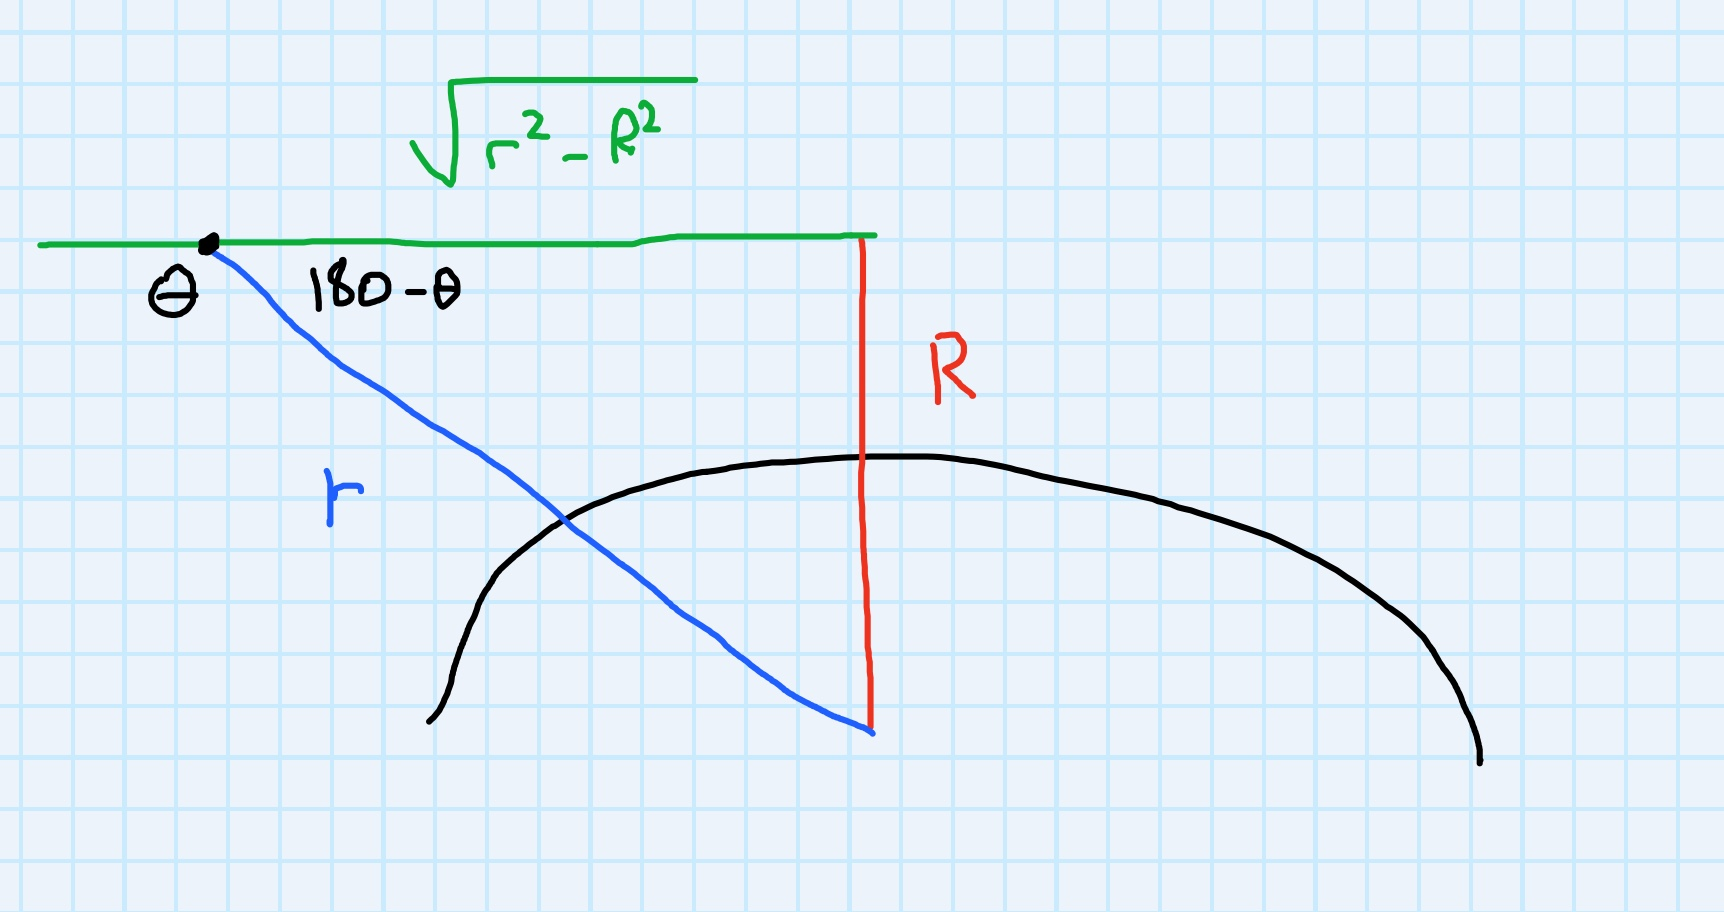
\includegraphics[width=12cm]{Screen Shot 2023-02-22 at 5.42.52 PM}
        \caption{My "Highly technical" attempt to illustrate the satellite's trajectory, with the satellite being marked by the black dot.}
        \label{fig:my_label}
\end{figure}
    
Thus, our integral becomes

    \begin{align*}
        \mathrm{GPE} &= GMm \cdot \int_{R}^{\infty} \frac{1}{r^2} \cdot -\frac{\sqrt{r^2-R^2}}{r} \, dr\\
        &= \frac{\sqrt{r^2-R^2}}{r^3} \, dr
    \end{align*}

    \newpage
    Making the substitution $r = R\sec(\theta)$, changing differentials, changing bounds, and simplifying gives us the integral:

    \begin{align*}
        \mathrm{GPE} &= -\frac{GMm}{R} \cdot \int_{0}^{\frac{\pi}{2}} \frac{\tan^2(\theta)}{\sec^2(\theta)} \, d\theta\\
        &= -\frac{GMm}{R} \cdot \int_{0}^{\frac{\pi}{2}} 1-\cos^2(\theta) \, d\theta\\
        &= -\frac{GMm}{R} \cdot \int_{0}^{\frac{\pi}{2}} \sin^2(\theta) \, d\theta\\
        &= -\frac{GMm}{R} \cdot \frac{\pi}{4}
    \end{align*}
    
    The final integral is solved using the cosine half-angle identity, and the computation is left to the reader


\section{Law of Conservation of Energy}
    \subsection{My Method}

    \begin{align*}
        E + GPE_i + KE_i &= 0\\
        E + -\frac{GMm}{R} \cdot \frac{\pi}{4} + \frac{1}{2}m(v_i)^2 &= 0\\
         E + -\frac{GMm\pi}{4R} + \frac{GMm}{2R} &= 0\\
         E &= \boxed{\frac{GMm}{2R}(\frac{\pi}{2}-1)}
    \end{align*}

    \subsection{My Teacher's Method}
    My teacher assumes the satellite is ejected out of orbit radially.
    \begin{align*}
        E + GPE_i + KE_i &= 0\\
        E + -\frac{GMm}{R} + \frac{1}{2}m(v_i)^2 &= 0\\
         E + -\frac{GMm}{R} + \frac{GMm}{2R} &= 0\\
         E &= \boxed{\frac{GMm}{2R}}
    \end{align*}

    


\end{document}
